% Options for packages loaded elsewhere
\PassOptionsToPackage{unicode}{hyperref}
\PassOptionsToPackage{hyphens}{url}
\documentclass[
]{article}
\usepackage{xcolor}
\usepackage[margin=1in]{geometry}
\usepackage{amsmath,amssymb}
\setcounter{secnumdepth}{-\maxdimen} % remove section numbering
\usepackage{iftex}
\ifPDFTeX
  \usepackage[T1]{fontenc}
  \usepackage[utf8]{inputenc}
  \usepackage{textcomp} % provide euro and other symbols
\else % if luatex or xetex
  \usepackage{unicode-math} % this also loads fontspec
  \defaultfontfeatures{Scale=MatchLowercase}
  \defaultfontfeatures[\rmfamily]{Ligatures=TeX,Scale=1}
\fi
\usepackage{lmodern}
\ifPDFTeX\else
  % xetex/luatex font selection
\fi
% Use upquote if available, for straight quotes in verbatim environments
\IfFileExists{upquote.sty}{\usepackage{upquote}}{}
\IfFileExists{microtype.sty}{% use microtype if available
  \usepackage[]{microtype}
  \UseMicrotypeSet[protrusion]{basicmath} % disable protrusion for tt fonts
}{}
\makeatletter
\@ifundefined{KOMAClassName}{% if non-KOMA class
  \IfFileExists{parskip.sty}{%
    \usepackage{parskip}
  }{% else
    \setlength{\parindent}{0pt}
    \setlength{\parskip}{6pt plus 2pt minus 1pt}}
}{% if KOMA class
  \KOMAoptions{parskip=half}}
\makeatother
\usepackage{longtable,booktabs,array}
\newcounter{none} % for unnumbered tables
\usepackage{calc} % for calculating minipage widths
% Correct order of tables after \paragraph or \subparagraph
\usepackage{etoolbox}
\makeatletter
\patchcmd\longtable{\par}{\if@noskipsec\mbox{}\fi\par}{}{}
\makeatother
% Allow footnotes in longtable head/foot
\IfFileExists{footnotehyper.sty}{\usepackage{footnotehyper}}{\usepackage{footnote}}
\makesavenoteenv{longtable}
\usepackage{graphicx}
\makeatletter
\newsavebox\pandoc@box
\newcommand*\pandocbounded[1]{% scales image to fit in text height/width
  \sbox\pandoc@box{#1}%
  \Gscale@div\@tempa{\textheight}{\dimexpr\ht\pandoc@box+\dp\pandoc@box\relax}%
  \Gscale@div\@tempb{\linewidth}{\wd\pandoc@box}%
  \ifdim\@tempb\p@<\@tempa\p@\let\@tempa\@tempb\fi% select the smaller of both
  \ifdim\@tempa\p@<\p@\scalebox{\@tempa}{\usebox\pandoc@box}%
  \else\usebox{\pandoc@box}%
  \fi%
}
% Set default figure placement to htbp
\def\fps@figure{htbp}
\makeatother
\setlength{\emergencystretch}{3em} % prevent overfull lines
\providecommand{\tightlist}{%
  \setlength{\itemsep}{0pt}\setlength{\parskip}{0pt}}
\usepackage{bookmark}
\IfFileExists{xurl.sty}{\usepackage{xurl}}{} % add URL line breaks if available
\urlstyle{same}
\hypersetup{
  hidelinks,
  pdfcreator={LaTeX via pandoc}}

\author{}
\date{}

\begin{document}

\section{\texorpdfstring{Thought Experiments through Chapter 5 of
\emph{Foundations of Quantum
Theory}}{Thought Experiments through Chapter 5 of Foundations of Quantum Theory}}\label{thought-experiments-through-chapter-5-of-foundations-of-quantum-theory}

\subsection{------From the Wall of Identification in Measurement to the
Rectangular Phase-Energy
Window}\label{from-the-wall-of-identification-in-measurement-to-the-rectangular-phase-energy-window}

\textbf{Author}: Noriaki Kihara, WF System Co., Ltd., ORCID:
\href{https://orcid.org/0009-0004-6753-4020}{0009-0004-6753-4020}
\textbf{Version}: v1.0 (incorporating multiple rounds of AI peer review:
Gemini × 1, Grok × 1, ChatGPT × 2) \textbf{Date}: May 2026
\textbf{Concept DOI}:
\href{https://doi.org/10.5281/zenodo.20398526}{10.5281/zenodo.20398526}
\textbf{v1 DOI}:
\href{https://doi.org/10.5281/zenodo.20398527}{10.5281/zenodo.20398527}
\textbf{Previous paper}: \emph{Thought Experiments through Chapter 3 of
Foundations of Quantum Theory} v3.0.1 (Concept DOI:
\href{https://doi.org/10.5281/zenodo.20391522}{10.5281/zenodo.20391522};
v3 DOI:
\href{https://doi.org/10.5281/zenodo.20393018}{10.5281/zenodo.20393018})
\textbf{License}: CC BY 4.0

\subsubsection{Abstract}\label{abstract}

Against the background of complex Hilbert space, observables,
measurement, uncertainty relations, the one-dimensional particle, the
box potential, and the tunneling effect developed in Chapters 1--5 of
Shimizu Akira's \emph{Foundations of Quantum Theory, New Edition}
{[}1{]}, we organize, through seven staged thought experiments,
measurement precision, uncertainty relations, wave packets, quantum
correlations, the algebra of observables, the ontology of physical
quantities, and the finite-width structure of particles into a unified
picture. Carrying over the five thought experiments of the previous
paper (\emph{Thought Experiments through Chapter 3} v3.0.1), this paper
adds, as the region corresponding to Chapters 4--5, the representation
of physical quantities over a complex phase space (Thought Experiment
VI) and the rereading of particles as rectangular phase-energy windows
with a central phase and a finite width (Thought Experiment VII). The
starting point is the ``wall of identification'' in classical metrology;
the terminal point is the ontological rereading ``a particle is a
rectangular phase-energy window with a central position phase and a
finite width, and the observed wave form appears as the Fourier
low-order partial sum of that window (the low-passed image in the
observation bandwidth).'' The core reading of this paper is the
semiclassical/geometric interpretation that positions phase-space
invariants as symplectic capacities, represented by de Gosson's quantum
blobs {[}9{]}. This paper does not modify the mathematical predictions
of standard quantum theory; within the scope of one-dimensional quantum
mechanics, measurement, uncertainty, and the box potential treated in
Chapters 1--5, it offers a conceptual rereading consistent with the
existing calculational formalism. For regions beyond Chapters 1--5 ---
Lorentz covariance, locality of fields, positivity, unitarity,
scattering amplitudes, spin statistics, gauge symmetry, particle
creation and annihilation --- whether the present rereading extends
consistently is reserved as an independent task. The paper does not deny
the Born rule. Rather, it treats the position-phase window
\(P_x(\theta)\) as a shape function, not a probability density. When the
observation system reads this shape function as the wave function
corresponding to a detection basis, the standard inner-product rule
\(p(a) = |\langle \varphi_a | \psi \rangle|^2\) then yields the
probability density.

\begin{center}\rule{0.5\linewidth}{0.5pt}\end{center}

\subsection{Thought Experiment I: The Wall of Identification in
Metrology}\label{thought-experiment-i-the-wall-of-identification-in-metrology}

\subsubsection{Setup}\label{setup}

Let a physical quantity \(A\) take real values. Using a
distance-concept-based ruler (returning only discrete values with
minimum spacing \(\Delta\)), we measure the distance \(L\) between two
points \(A_1, A_2\).

In each measurement, one of the two adjacent grid points
\(\{k\Delta, (k+1)\Delta\}\) enclosing the true value is returned, with
probabilities determined by the in-cell position \(r\) of the true
value:

P(upper) = \(r/\Delta\), P(lower) = \(1 - r/\Delta\)

(position-dependent dithering).

\subsubsection{Behavior of the N-fold
average}\label{behavior-of-the-n-fold-average}

When \(A_1 = A_2\), the single-measurement distance
\(D = \varepsilon_2 - \varepsilon_1\) takes values
\(\{-\Delta, 0, +\Delta\}\). Writing the in-cell position of the true
value as \(q = r/\Delta \in [0, 1]\), in general:

\begin{itemize}
\tightlist
\item
  \(P(D = +\Delta) = q(1-q)\)
\item
  \(P(D = -\Delta) = q(1-q)\)
\item
  \(P(D = 0) = q^2 + (1-q)^2\)
\end{itemize}

Hence \(E[D] = 0\), \(\mathrm{Var}[D] = 2q(1-q)\Delta^2\),
\(\sigma_D = \sqrt{2q(1-q)}\cdot\Delta\).

In particular, at the symmetric position \(q = 1/2\) the probability
distribution becomes \(\{1/4, 1/2, 1/4\}\), with
\(\mathrm{Var}[D] = \Delta^2/2\) and \(\sigma_N = \Delta/\sqrt{2N}\).

As \(N \to \infty\), \(\sigma_N \to 0\) and \(\hat{L}_N \to L\) with
probability 1.

\subsubsection{Condition for
distinguishability}\label{condition-for-distinguishability}

To recognize \(A_1\) and \(A_2\) as two distinct objects, both must
belong to different \(\Delta\)-cells. If they fall within the same cell,
the ruler cannot tell ``one point or two,'' and the quantity ``distance
between two points'' does not arise.

The condition for the distance-measurement problem to be well-posed is
therefore

\[L \geq \Delta.\]

The region \(L < \Delta\) is not ``buried in measurement error'' but a
region in which the very concept of ``two points'' is undefined.

\subsubsection{Conclusion}\label{conclusion}

\begin{quote}
When measuring distance with a distance-concept-based ruler, any metric
below the ruler spacing \(\Delta\) is \textbf{measurement-undefined}
even before invoking the uncertainty relation. \(\Delta\) acts not as a
resolution but as the threshold of individuation.

Within the range \(L \geq \Delta\), infinitely many measurements can
attain arbitrary precision regardless of the absolute value of
\(\Delta\).
\end{quote}

This argument holds for any distance-concept-based ruler and is
structurally analogous to, but independent of, the minimum-length
discussion in quantum gravity at the Planck scale {[}10{]}.

\textbf{The relation between epistemic and ontological limits}: The
``undefined'' above is not the ontological claim that distances below
\(\Delta\) \textbf{do not exist} (that space is discretized). It is the
claim that, viewed from inside an observation system built on a ruler of
spacing \(\Delta\), two points are \textbf{epistemically
indistinguishable, and within that observation system there is no
operational meaning to treating them as anything other than
ontologically identical} --- that is, an epistemic limit manifests as a
geometric one. Thus our position is not to place epistemology and
ontology side by side as independent, but to take the limit of
distinctions constructible inside the observation system to be the
geometric limit of individuation: an epistemology-led geometry. From
this viewpoint, the external question ``is the real space discrete or
continuous?'' is not entered.

\textbf{More precisely}: Rather than the ontological phrasing ``two
points do not exist below \(\Delta\),'' the formulation ``no projection
operator distinguishes two points in the observational algebra generated
by a \(\Delta\)-spaced ruler'' is more appropriate as a connection to
quantum measurement theory. This discussion can be made consistent with
the framework of generalized measurements via POVMs / Kraus operators,
and positioned as a special case of coarse-grained measurement.

Note that when \(A_1, A_2\) are externally pre-labeled as distinct
objects, sub-cell precision can be estimated from the mean difference
via repeated measurement (N → ∞ convergence by position-dependent
dithering). ``Undefined'' here refers to the case where no operation
exists, inside the observation system, to individuate the two objects.

\begin{center}\rule{0.5\linewidth}{0.5pt}\end{center}

\subsection{Thought Experiment II: The Locus of
Fluctuation}\label{thought-experiment-ii-the-locus-of-fluctuation}

\subsubsection{Setup}\label{setup-1}

Consider the reverse situation. The ruler has infinite precision and
returns the input value as-is. On the other hand, the physical quantity
\(A\) itself fluctuates around its true value \(A'\) as

\(A_i = A' + \xi_i\),
\(\xi_i \sim \mathrm{Uniform}[-\Delta/2, +\Delta/2]\).

Assume \(L > \Delta\).

\subsubsection{N-fold average}\label{n-fold-average}

\begin{itemize}
\tightlist
\item
  \(E[\hat{L}_N] = A'\)
\item
  \(\mathrm{Var}[L_i] = \Delta^2/12\)
\item
  \(\sigma_N = \Delta/\sqrt{12N} \to 0\)
\end{itemize}

\subsubsection{Comparison with Thought Experiment
I}\label{comparison-with-thought-experiment-i}

Concretizing both cases with true value 7.7 and spacing \(\Delta = 1\),
both yield the same empirical distribution: ``in 100 measurements, 7
appears about 30 times, 8 about 70 times, and the mean converges to
7.7.''

{\def\LTcaptype{none} % do not increment counter
\begin{longtable}[]{@{}
  >{\raggedright\arraybackslash}p{(\linewidth - 4\tabcolsep) * \real{0.3333}}
  >{\raggedright\arraybackslash}p{(\linewidth - 4\tabcolsep) * \real{0.3333}}
  >{\raggedright\arraybackslash}p{(\linewidth - 4\tabcolsep) * \real{0.3333}}@{}}
\toprule\noalign{}
\begin{minipage}[b]{\linewidth}\raggedright
\end{minipage} & \begin{minipage}[b]{\linewidth}\raggedright
Fluctuation on the ruler side
\end{minipage} & \begin{minipage}[b]{\linewidth}\raggedright
Fluctuation on the physical-quantity side
\end{minipage} \\
\midrule\noalign{}
\endhead
\bottomrule\noalign{}
\endlastfoot
Single-output space & Discrete \(\{k\Delta, (k+1)\Delta\}\) &
Continuous \\
Probability distribution & Position-dependent Bernoulli & Sum of
uniforms \\
\(N \to \infty\) limit & True value & True value \\
Distinguishable from data & Impossible & \\
\end{longtable}
}

\subsubsection{Two-sided fluctuation}\label{two-sided-fluctuation}

In the general case where physical-side fluctuation \(\xi\) (width
\(\delta\)) and ruler-side fluctuation \(\eta\) (width \(\sigma\))
coexist independently:

\begin{itemize}
\tightlist
\item
  Observed value \(L_i = A' + \xi_i + \eta_i\)
\item
  \(\sigma_N = \sqrt{\mathrm{Var}[\xi] + \mathrm{Var}[\eta]} / \sqrt{N} \to 0\)
\end{itemize}

The \(1/\sqrt{N}\) decay is preserved, but separating \(\delta\) and
\(\sigma\) from a single observed series requires additional assumptions
outside the observation (independent calibration of the ruler,
time-series decomposition, prior knowledge of distributional form,
etc.).

\subsubsection{Conclusion}\label{conclusion-1}

\begin{quote}
Define the observed magnitude of fluctuation as
\(\Delta_{\mathrm{obs}}\). Whether it comes from the quantization width
of the ruler, from the fluctuation of the physical quantity itself, or
from their combination, cannot be decided from the observed data alone.

What can be stated rigorously is not ``convergence to an objective true
value'' but ``convergence to an effective true value defined by the
observer,'' together with the \(1/\sqrt{N}\) decay.
\end{quote}

\textbf{More precisely}: ``Cannot be decided from observed data alone''
means ``under the conditions of a single observation series, a single
measurement setting, and no prior calibration.'' When the apparatus
Hamiltonian is known, it is theoretically possible to distinguish
system-side fluctuation from environment- (apparatus-) side fluctuation
via decoherence theory for open quantum systems. The claim of this paper
is restricted to non-identifiability from observation data alone, and
connects to epistemic aspects (QBist interpretation) that depend on the
observer's knowledge state.

\begin{center}\rule{0.5\linewidth}{0.5pt}\end{center}

\subsection{Thought Experiment III: Wavelength Representation of
Momentum and the Uncertainty
Relation}\label{thought-experiment-iii-wavelength-representation-of-momentum-and-the-uncertainty-relation}

\subsubsection{Setup}\label{setup-2}

Extend the object of Thought Experiment II to a quantum wave packet. For
position \(x\), consider the center of the wave packet (expectation
value \(\langle x \rangle\)) \(x_1\) and the spread \(\delta x\). Here
the ``center'' is a label of the wave packet's distribution; we do not
take the stance that there is an objective true value outside the
observation.

Similarly, for momentum \(p\), consider the center (expectation value
\(\langle p \rangle\)) \(p_1\) and the spread \(\delta p\).

\subsubsection{Rewriting via wavelength}\label{rewriting-via-wavelength}

The de Broglie relation {[}2{]}:

\[p = \frac{h}{\lambda} = \hbar k, \quad k = \frac{2\pi}{\lambda}\]

gives the fluctuation of momentum as

\[|\delta p| = \frac{h}{\lambda^2}|\delta\lambda| = \hbar \, |\delta k|\]

(the differential relation \(dp/d\lambda = -h/\lambda^2\) has its sign
absorbed in taking absolute values for the fluctuation width).

Rewriting the uncertainty relation \(\Delta x \Delta p \geq \hbar/2\)
{[}7{]} in wave-number form:

\[\Delta x \cdot \Delta k \geq \frac{1}{2}.\]

\subsubsection{Observation}\label{observation}

In this form, Planck's constant \(\hbar\) disappears from both sides of
the inequality. What remains is the mathematical Fourier inequality on
the product of position and wave-number.

Planck's constant \(\hbar\) functions as a dimensional conversion factor
connecting units of position (m) and momentum (kg·m/s). A similar view,
treating Planck's constant not as an observable but as a unit-choice
convention, has been presented by Ralston {[}8{]}.

Qualitatively:

\begin{itemize}
\tightlist
\item
  Determining position precisely ⟺ narrowing the position wave packet ⟺
  broadening the wavelength distribution ⟺ momentum becomes vague
\item
  Determining momentum precisely ⟺ narrowing to a single wavelength ⟺
  spreading throughout space ⟺ position becomes vague
\end{itemize}

{\def\LTcaptype{none} % do not increment counter
\begin{longtable}[]{@{}lll@{}}
\toprule\noalign{}
Form of the wave packet & Spatial extent & Wavelength distribution \\
\midrule\noalign{}
\endhead
\bottomrule\noalign{}
\endlastfoot
Delta function & \(\delta x = 0\) & All wavelengths \\
Rectangular pulse & Finite & Sinc function \\
Pure sine wave & Whole space & Single wavelength \\
\end{longtable}
}

\subsubsection{Conclusion}\label{conclusion-2}

\begin{quote}
In the wave-number representation, the position-momentum uncertainty
relation becomes \(\Delta x \Delta k \geq 1/2\), the lower bound on the
product of conjugate quantities in the Fourier transform. Planck's
constant appears as a dimensional conversion factor.
\end{quote}

\textbf{More precisely}: \(\hbar\) is the action quantum appearing in
the canonical commutation relation \([x, p] = i\hbar\); this physical
content is independent of the fact that it can be set to \(\hbar = 1\)
in natural units. The claim here is restricted to the rewriting: in the
wave-number representation the canonical commutation relation becomes
\([x, k] = i\), and the uncertainty relation can be reread as the
geometric inequality of wave-number conjugacy. ``\(\hbar\) disappears''
means it disappears from the surface of the description, not that the
physical role of \(\hbar\) as a quantum of action is denied.

\begin{center}\rule{0.5\linewidth}{0.5pt}\end{center}

\subsection{Thought Experiment IV: Quantum Correlation as a Composite
Wave
Packet}\label{thought-experiment-iv-quantum-correlation-as-a-composite-wave-packet}

\subsubsection{Setup}\label{setup-3}

Consider a state localized in two spatial regions \(A, B\) and
correlated via a common conserved quantity (momentum, energy, etc.).
This is the system standardly described as a ``two-particle entangled
state'' {[}3, 4, 5{]}.

We attempt to describe it as ``a single composite wave packet localized
in two regions in space.''

\subsubsection{The string metaphor}\label{the-string-metaphor}

A long, tensioned string vibrating on a baseline. If one end is suddenly
fixed, a soliton-like deformation appears at the opposite end. This is
the consequence of the whole string obeying conservation laws as one
system; no information has propagated from one end to the other.

\subsubsection{Geometry of the composite wave
packet}\label{geometry-of-the-composite-wave-packet}

\begin{itemize}
\tightlist
\item
  A composite wave packet occupies a single area element in phase space.
\item
  In space, it has two localized peaks in regions \(A, B\).
\item
  A local interaction on side \(A\) shrinks \(\Delta x_A\).
\item
  By the Robertson inequality {[}6{]} and Robertson--Schrödinger-type
  covariance constraints, when the spread along the projection direction
  on side \(A\) shrinks, a compensatory change appears in the conjugate
  direction or in covariance components, broadening \(\Delta p_A\).
\item
  To satisfy the geometric constraint on the whole composite wave packet
  --- the symplectic capacity --- the spread of side \(B\)'s wave packet
  also deforms geometrically.
\end{itemize}

However, the deformation on side \(B\) is a change in the description of
the post-state conditioned on side-\(A\)'s measurement outcome; the
unconditioned reduced density matrix of side \(B\) alone does not change
under local operations on side \(A\). This distinction is consistent
with the no-signalling theorem of standard quantum theory.

In this description, no information transmission from \(A\) to \(B\) is
introduced. The observed correlations are a geometric consequence
reflecting the state of the whole system together with conservation
laws, symmetries, and symplectic capacity constraints.

\subsubsection{The geometric invariant}\label{the-geometric-invariant}

What constrains the geometry of the composite system is not individual
wavelengths or positions but the \textbf{symplectic capacity} formed by
the product of the spreads of conjugate observables (the area element in
phase space):

\[\Delta x \cdot \Delta p \geq \frac{\hbar}{2}, \quad \Delta A \cdot \Delta B \geq \frac{1}{2}\left|\langle [A,B] \rangle\right|\]

The left-hand side has the dimension of area, and the inequality denotes
the lower bound on area. This is not a simple conservation law for
\(\Delta x \Delta p\) but a geometric constraint by the symplectic
capacity invariant under canonical transformations.

Strictly speaking, in multi-degree-of-freedom systems the symplectic
capacity is not defined as the total phase-space volume or as the
product of individual uncertainty products, but as a symplectic
invariant for projections onto canonical 2-planes (Gromov's
non-squeezing theorem {[}15{]}). We use the \(\Delta x \Delta p\)-type
area element as an intuitive shadow conveying the essence.

\subsubsection{Conclusion}\label{conclusion-3}

\begin{quote}
Quantum correlations can be understood through the geometric picture
``reading a single composite state as projections onto multiple regions
in space.'' The observed correlations are a geometric consequence
reflecting the state of the whole system, conservation laws and
symmetries, and symplectic capacity constraints; this description
requires no information transmission between spatially separated
systems.
\end{quote}

\textbf{More precisely}: The composite-wave-packet picture in this paper
is an attempt to read a single state vector on a tensor-product Hilbert
space (in standard quantum theory) through the geometric intuition of
phase space. The soliton-string analogy is an intuitive presentation of
the geometric structure of conservation laws and is not a complete
re-derivation of quantitative predictions such as the maximum
Bell-inequality violation \(2\sqrt{2}\) (the Tsirelson bound) of the
CHSH inequality. Those quantitative predictions are derived from the
algebraic structure of quantum theory independently of the classical
wave analogy. The ``no information transmission'' point is consistent
with the no-signalling theorem of standard quantum theory (partial trace
of density operators, invariance under local operations).

\begin{center}\rule{0.5\linewidth}{0.5pt}\end{center}

\subsection{Thought Experiment V: The Algebra of
Observables}\label{thought-experiment-v-the-algebra-of-observables}

\textbf{Preface on the scope of the metaphor}: This section uses
intuitive terms such as ``wave packet,'' ``area element,'' and
``projection.'' These serve as valid metaphors for the
semiclassical/geometric interpretation of pure states in the
position--momentum system (infinite-dimensional, continuous spectrum).
In spin systems or finite-dimensional systems, the wave packet must be
reread as a ``point on projective Hilbert space, a state direction,''
and the area element as the ``geometry of the non-commutative algebra
generated by projection operators.'' Each thought experiment's closing
``More precisely'' section supplies the rigorous mathematical
correspondence.

\subsubsection{Setup}\label{setup-4}

Enumerate several pairs of physical quantities obeying the uncertainty
relation \(\Delta A \Delta B \geq |\langle [A,B] \rangle|/2\):

\begin{itemize}
\tightlist
\item
  Position \(x\) ↔ momentum \(p\)
\item
  Spin \(S_x\) ↔ \(S_y\) ↔ \(S_z\)
\item
  Polarization (H/V ↔ D/A ↔ R/L)
\item
  Angular momentum \(L_x\) ↔ \(L_y\) ↔ \(L_z\)
\item
  Energy ↔ time (note: the energy-time uncertainty has a different
  mathematical status from Robertson-type uncertainties between
  position-momentum or spin components, since time in ordinary quantum
  mechanics is not defined as a self-adjoint operator)
\end{itemize}

All of these share a common structure.

\subsubsection{Common structure}\label{common-structure}

{\def\LTcaptype{none} % do not increment counter
\begin{longtable}[]{@{}
  >{\raggedright\arraybackslash}p{(\linewidth - 4\tabcolsep) * \real{0.3333}}
  >{\raggedright\arraybackslash}p{(\linewidth - 4\tabcolsep) * \real{0.3333}}
  >{\raggedright\arraybackslash}p{(\linewidth - 4\tabcolsep) * \real{0.3333}}@{}}
\toprule\noalign{}
\begin{minipage}[b]{\linewidth}\raggedright
Pair of observables
\end{minipage} & \begin{minipage}[b]{\linewidth}\raggedright
Shared structure
\end{minipage} & \begin{minipage}[b]{\linewidth}\raggedright
Role of distinct operators
\end{minipage} \\
\midrule\noalign{}
\endhead
\bottomrule\noalign{}
\endlastfoot
\(x\) ↔ \(p\) & Area element in phase space & Direct coordinate ↔
Fourier coordinate \\
\(S_x\) ↔ \(S_y\) ↔ \(S_z\) & Area element in spin phase space &
Projections onto different axes \\
Polarization bases & Area element on the polarization plane &
Projections onto different bases \\
\(L_x\) ↔ \(L_y\) ↔ \(L_z\) & Angular-momentum phase space & Projections
onto different axes \\
\(E\) ↔ \(t\) & Energy-time phase space & Different representations \\
\end{longtable}
}

\subsubsection{Unified picture}\label{unified-picture}

In complex Hilbert space:

{\def\LTcaptype{none} % do not increment counter
\begin{longtable}[]{@{}
  >{\raggedright\arraybackslash}p{(\linewidth - 2\tabcolsep) * \real{0.5000}}
  >{\raggedright\arraybackslash}p{(\linewidth - 2\tabcolsep) * \real{0.5000}}@{}}
\toprule\noalign{}
\begin{minipage}[b]{\linewidth}\raggedright
Formal object
\end{minipage} & \begin{minipage}[b]{\linewidth}\raggedright
Geometric interpretation
\end{minipage} \\
\midrule\noalign{}
\endhead
\bottomrule\noalign{}
\endlastfoot
Eigenvector \(|\psi\rangle\) & Wave packet (a single area element in
phase space) \\
Operator \(\hat{A}\) & Projection extracting a real value from the area
element \\
Eigenvalue \(a\) & The result of the projection \\
Non-commutativity \([\hat{A}, \hat{B}] \neq 0\) & Two projections
viewing the same area element from different directions \\
\end{longtable}
}

\subsubsection{Conclusion}\label{conclusion-4}

\begin{quote}
Observables obeying an uncertainty relation are described as different
projections of the same wave packet (eigenvector). The product of
non-commuting projections has the area element of the wave packet as a
lower bound (Robertson inequality).

In this paper's geometric reading, observables are understood as
quantities that extract real-valued distributions from states, with
values obtained through measurement bases or spectral projections. The
wave packet, in the semiclassical phase-space representation, is
interpreted as an area element, whose spread is restricted by the
Robertson--Schrödinger-type covariance constraint and by the symplectic
capacity. The projections of observables do not take arbitrary
independent values: they are correlated under the geometric invariant of
the same state.
\end{quote}

The area-element picture of this paper is consistent with de Gosson's
{[}9{]} quantum blob (the minimum unit of phase space corresponding to
the Robertson--Schrödinger minimum uncertainty, measured as a symplectic
capacity --- an area-type invariant on canonical 2-planes). This paper
is positioned as a reconstruction of de Gosson's mathematically heavy
symplectic-geometric framework in the intuitive form of a thought
experiment as a reading of Chapter 1 of Shimizu's textbook. Related
geometric formulations include the Ashtekar--Schilling formulation based
on the Kähler structure of projective Hilbert space {[}11{]} and the
algebraic approach treating the algebra of observables as primary
{[}12{]}.

\textbf{More precisely}: ``Operator = projection'' can be confused with
the specific notion of a projection operator. It is more appropriate to
say that observables are self-adjoint operators, and in projective
measurements values are extracted via spectral projections (in
generalized measurements, POVMs). ``Eigenvector = wave packet'' is a
useful metaphor for position-momentum systems; in spin systems or
finite-dimensional systems, it should be read as a ``state direction, a
point on projective Hilbert space.'' The phase-space area-element
picture in this paper is a semiclassical/geometric interpretation;
rigorous purely-Hilbert-space formulations are provided by Weyl
quantization, the Wigner function {[}13{]}, the Moyal bracket {[}14{]},
and geometric quantization.

Note also that the Robertson inequality itself is a lower-bound
condition; there is no general absolute upper bound on
\((\Delta x)(\Delta p)\) for position-momentum in infinite-dimensional
Hilbert space (for a free particle's Gaussian wave packet, \(\Delta x\)
can increase with time). However, in finite-dimensional systems, with
bounded observables, or in state-dependent contexts, upper-bound-type
uncertainty relations --- ``reverse uncertainty relations'' --- have
been studied in recent years. The claim of this paper about geometric
invariants is most accurately read not as a simple conservation law for
\(\Delta x \Delta p\) but as the invariance of the symplectic capacity
under canonical transformations (de Gosson's quantum blob {[}9{]}).

\begin{center}\rule{0.5\linewidth}{0.5pt}\end{center}

\subsection{Thought Experiment VI: Are Physical Quantities Real Numbers?
--- Physical Quantities as Quantities over a Complex Phase
Space}\label{thought-experiment-vi-are-physical-quantities-real-numbers-physical-quantities-as-quantities-over-a-complex-phase-space}

\subsubsection{Terminology note: on ``complex phase
space''}\label{terminology-note-on-complex-phase-space}

By ``complex phase space'' we mean not a single standardized term but a
\textbf{working umbrella term for complex-phase structures} appearing
commonly across complex Hilbert space \(\mathcal{H}\), the Kähler
structure of projective Hilbert space \(\mathbb{P}(\mathcal{H})\), the
Wigner--Moyal phase space, and the phase factor \(e^{i\theta}\). The
strict mathematical object referred to differs by context, but the
common feature --- ``real projections back a complex-phase structure''
--- is captured by this convenient name.

\subsubsection{Setup}\label{setup-5}

Through Thought Experiments I--V, we reached an algebraic picture in
which observables are described as different projections of the same
wave packet. Here we invert the question: what is the substance of a
physical quantity \emph{before} it is projected? Does the fact that
observed values are real numbers imply that the underlying structure of
physical quantities is closed over the real-number field?

\subsubsection{Three assumptions}\label{three-assumptions}

We assume the following.

\textbf{Assumption 1}: Observed physical quantities are real-valued.
However, this is a constraint on the output type of the observation
operation and does not imply that the underlying structure generating
the quantity is closed over the reals. Just as wave functions are
complex while observed probabilities are real, even if what is observed
is real, we allow the underlying generating structure to be complex.

\textbf{Assumption 2}: Fundamental physical quantities are defined as
quantities over a complex-valued phase space. Real-valued observed
values appear as real projections of that complex-phase structure (real
part, absolute value, functional value, etc.):

\[
\mathcal{L} = \mathcal{L}(z, \bar{z}), \quad L_{\mathrm{obs}} = F(\mathcal{L}, \bar{\mathcal{L}}) \in \mathbb{R}
\]

\textbf{Assumption 3}: Physically stable values are selected not as
continuous arbitrary values but as discrete values satisfying a
phase-closure condition (the phase closes consistently across the
system). One-dimensionally this is the standing-wave condition
\(L = n\lambda/2\); in phase space, it corresponds to the
Bohr--Sommerfeld / EBK quantization condition
\(\oint p\, dq = 2\pi\hbar(n + \mu/4)\) for the action integral
{[}16{]}; more generally, it corresponds to the integrality condition
\([\omega]/(2\pi\hbar) \in H^2(M, \mathbb{Z})\) of geometric
quantization. At boundaries and turning points, Maslov phase corrections
of \(\pi/2\) units appear.

\subsubsection{Complex representation of the position
phase}\label{complex-representation-of-the-position-phase}

Representing position \(x\) as a phase \(\theta_x = kx\), the central
position \(x_0\) corresponds to the central phase \(\theta_x = kx_0\),
and the spatial spread \(\Delta x\) corresponds to the phase width
\(\Delta\theta_x = k\Delta x\).

\begin{figure}
\centering
\pandocbounded{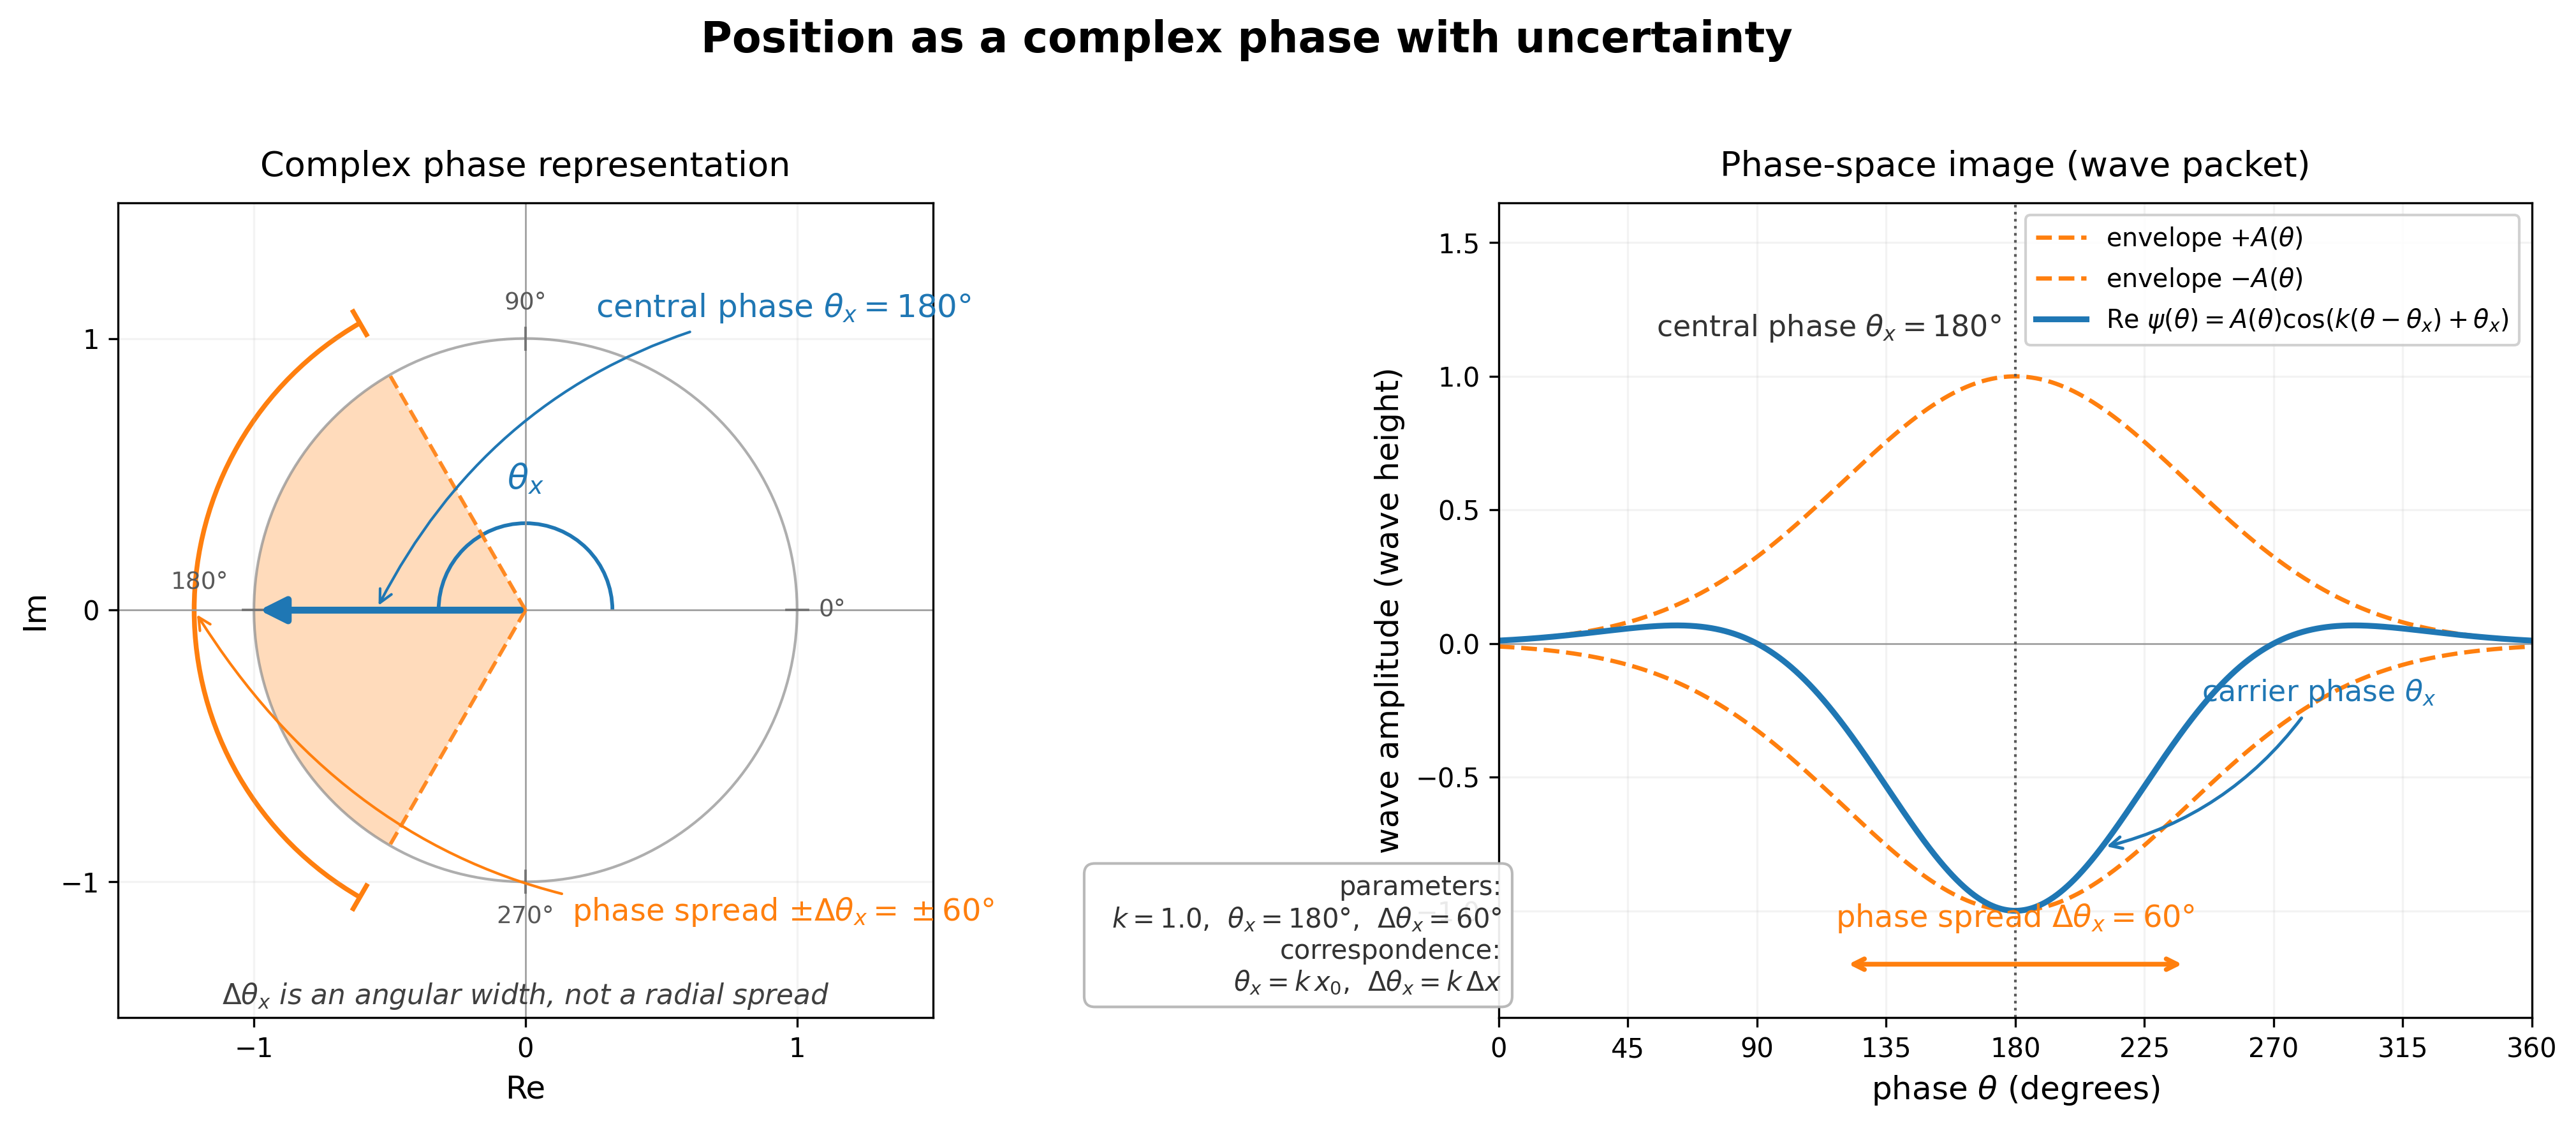
\includegraphics[keepaspectratio,alt={Complex representation of the position phase and phase-space image}]{figures/phase_position_wavepacket.png}}
\caption{Complex representation of the position phase and phase-space
image}
\end{figure}

\textbf{Figure VI-1}: Complex representation of the position phase and
phase-space image. The left panel shows, on the complex plane, the
central phase \(\theta_x = 180°\) and the surrounding angular width
\(\pm\Delta\theta_x = 60°\). \(\Delta\theta_x\) is an angular width, not
a radial spread. The right panel shows the same structure as a wave
packet on the phase axis \(\theta\), with the real part of
\(\mathrm{Re}\,\psi(\theta) = A(\theta)\cos(k(\theta-\theta_x)+\theta_x)\)
as a thick line and the envelopes \(\pm A(\theta)\) as dashed lines. The
two panels are connected by the correspondence
\(\theta_x = kx_0,\ \Delta\theta_x = k\Delta x\).

\subsubsection{Connection to existing
theories}\label{connection-to-existing-theories}

This model connects to existing quantum geometry:

\begin{itemize}
\tightlist
\item
  \textbf{Quantum geometric tensor} {[}18{]}:
  \(Q_{ij} = g_{ij} + (i/2)\Omega_{ij}\), where the real part is a
  distance (Provost--Vallée / Fubini--Study metric) and the imaginary
  part is the Berry curvature (symplectic structure, non-commutativity).
\item
  \textbf{Complex Hilbert space and projective space} {[}11{]}: physical
  states are treated as rays, and projective space
  \(\mathbb{P}(\mathcal{H})\) naturally becomes a Kähler manifold.
\item
  \textbf{Wigner--Moyal formalism} {[}13, 14{]}: quantum theory
  described as a pseudo-probability distribution on phase space.
\item
  \textbf{Non-Hermitian / PT-symmetric quantum theory} {[}19{]}:
  self-adjointness of observables is not adopted as a foundational
  axiom; real observed values are recovered through an appropriate inner
  product and metric operator.
\item
  \textbf{Ralston (2020)} {[}8{]}: Planck's constant is treated not as
  an observable but as a unit-choice convention.
\end{itemize}

\subsubsection{Conclusion}\label{conclusion-5}

\begin{quote}
The substance of a physical quantity can be read not as a single value
on the real line but as a phase-closure structure on a complex phase
space. Under this assumption, uncertainty, interference, entanglement,
and quantization are not separate phenomena but the same structure seen
through different observation projections.
\end{quote}

\textbf{More precisely}: This hypothesis is not a new predictive theory
but an ontological/conceptual reinterpretation of existing quantum
theory. The mathematical predictions of standard quantum theory are not
changed. What breaks down when complex structure is placed on the side
of substance is, e.g., the standard measurement theory based on
self-adjointness of observables as a foundational axiom, complex-time
QFT without reflection positivity, or a complexified standard model that
fails to recover a unitary S-matrix {[}20{]}. These break-downs do not
mean ``complex structure itself is bad'' but indicate that projection
rules onto real observables, positivity, and unitarity must be recovered
separately. The study by Renou et al.~(2021) {[}21{]} on experimental
distinction between real-number and complex-number versions of quantum
theory points toward the direction of experimentally testing the
physical necessity of complex structure.

\begin{center}\rule{0.5\linewidth}{0.5pt}\end{center}

\subsection{Thought Experiment VII: Are Particles Rectangular
Phase-Energy Windows? --- A Rereading of the One-Dimensional Particle
and the Box
Potential}\label{thought-experiment-vii-are-particles-rectangular-phase-energy-windows-a-rereading-of-the-one-dimensional-particle-and-the-box-potential}

\subsubsection{Setup}\label{setup-6}

We perform the thought experiment of rereading the one-dimensional
particle, the well potential, the box potential, and the tunneling
effect treated in Chapter 5 of Shimizu's \emph{Foundations of Quantum
Theory} (and similar one-dimensional quantum-mechanics textbooks) ---
not as the behavior of a particle under external conditions but as the
foundational image of the particle itself.

\subsubsection{Position phase as a rectangular phase
window}\label{position-phase-as-a-rectangular-phase-window}

In Thought Experiment VI the position phase was introduced as a quantity
over a complex phase space. To give a more concrete form, we place the
position phase as a rectangular phase window:

\[
R_x(\theta) = \begin{cases}
1, & |\theta - \theta_x| \leq \dfrac{\Delta\theta_x}{2}, \\
0, & |\theta - \theta_x| > \dfrac{\Delta\theta_x}{2}.
\end{cases}
\]

Here \(\theta_x\) is the central phase and \(\Delta\theta_x\) is the
full width of the window. The value is 1 in the region
\(|\theta - \theta_x| \leq \Delta\theta_x/2\) and 0 elsewhere. This is
the \textbf{body} of the particle / position phase.

\subsubsection{The observation image as a Fourier partial
sum}\label{the-observation-image-as-a-fourier-partial-sum}

Expand the rectangular phase window \(R_x(\theta)\) in a Fourier series
of period \(2\pi\), and define the observation-bandwidth low-pass
operator \(L_\Lambda\) as ``the operation truncating at the \(N\)-th
harmonic.'' The observation image is

\[
P_x^{\mathrm{obs}}(\theta) = L_\Lambda[R_x(\theta)] = S_N(\theta) = \frac{a_0}{2} + \sum_{n=1}^{N} a_n \cos\bigl(n(\theta - \theta_x)\bigr)
\]

where the Fourier coefficients are (even expansion about the center
\(\theta_x\)):

\[
a_0 = \frac{\Delta\theta_x}{\pi}, \quad a_n = \frac{2}{n\pi}\sin\!\left(\frac{n\Delta\theta_x}{2}\right) \quad (n \geq 1).
\]

\begin{figure}
\centering
\pandocbounded{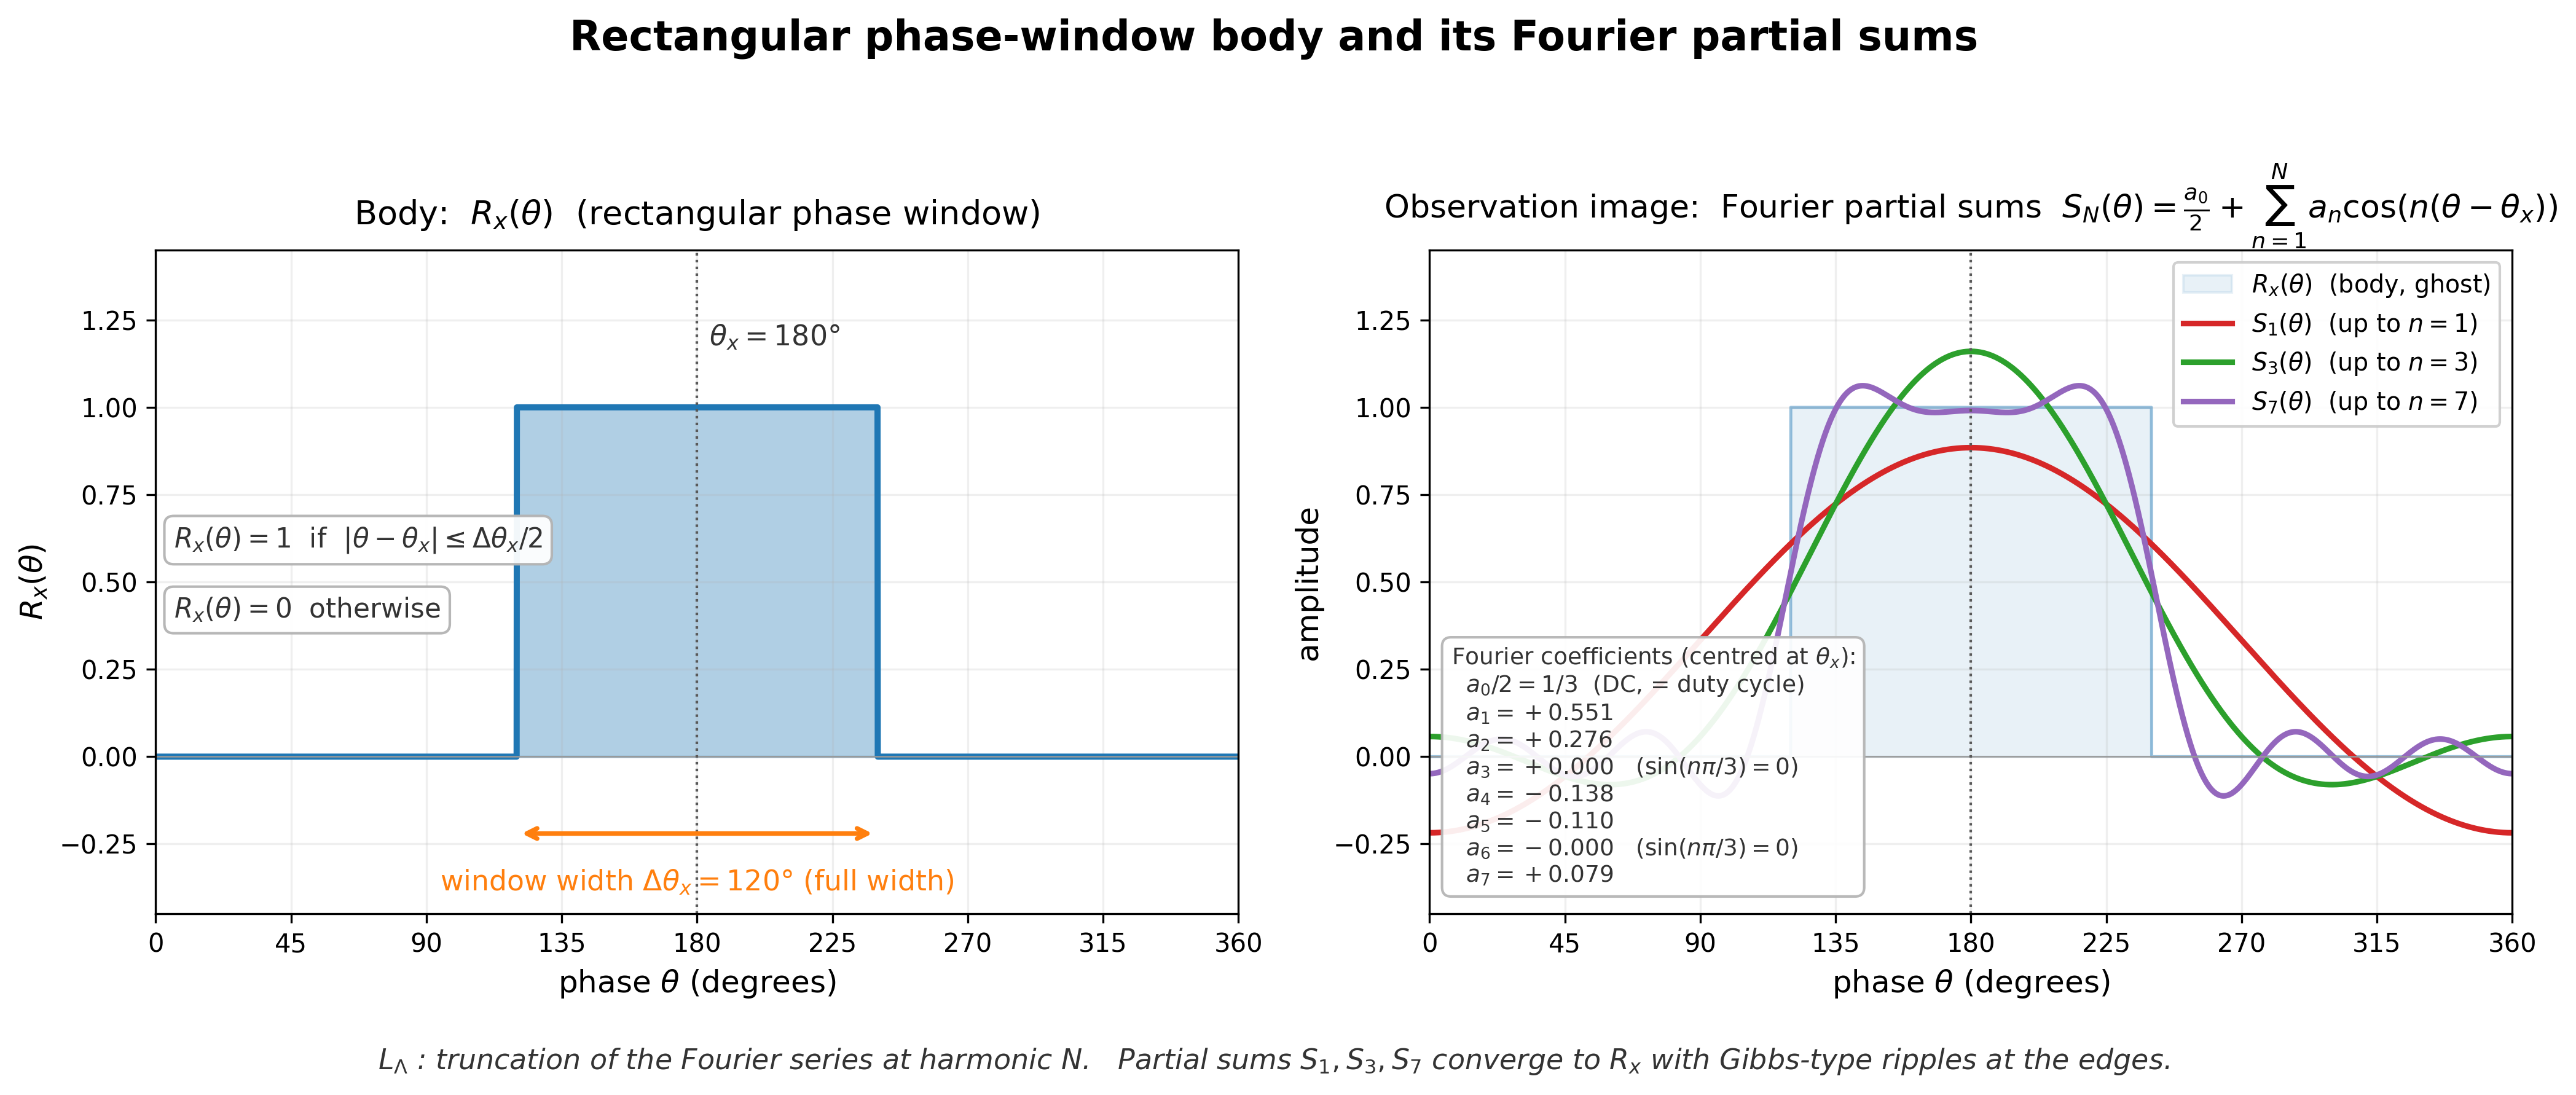
\includegraphics[keepaspectratio,alt={Body of the rectangular phase window and its Fourier partial sums}]{figures/phase_window_body_and_observation.png}}
\caption{Body of the rectangular phase window and its Fourier partial
sums}
\end{figure}

\textbf{Figure VII-1}: The body of the rectangular phase window
\(R_x(\theta)\) (left) and its observation image as Fourier partial sums
\(S_N(\theta)\) (right). The left panel shows the underlying form, the
rectangular phase window \(R_x(\theta)\) (center \(\theta_x = 180°\),
full width \(\Delta\theta_x = 120°\)). The right panel shows the partial
sums \(S_N(\theta)\) truncating the Fourier series at the \(N\)-th
harmonic, for \(N = 1, 3, 7\). For \(\Delta\theta_x = 120° = 2\pi/3\):
\(a_0/2 = 1/3\) (duty cycle), \(a_1 \approx +0.55\),
\(a_2 \approx +0.28\), \(a_3 = 0\) (zero of \(\sin(n\pi/3)\)),
\(a_4 \approx -0.14\), \(a_5 \approx -0.11\), \(a_7 \approx +0.08\). The
low-pass operator \(L_\Lambda\) corresponds to truncating the Fourier
series at the \(N\)-th harmonic; as \(N\) grows the partial sums
converge to the rectangle (with Gibbs-type ringing at discontinuities).
The lowest order \(S_1\) consists of the DC term \(a_0/2 = 1/3\) and the
first cosine harmonic \(a_1 \cos(\theta - \theta_x)\).

Strictly speaking, when treating an observation image of a rectangular
window with bandwidth limitation, not only Fourier partial sums but also
the prolate spheroidal wave functions (PSWF) of Slepian--Pollak {[}31{]}
and Landau--Pollak {[}32{]} --- which optimize the simultaneous
concentration of time width and bandwidth --- appear naturally.
Moreover, by Hardy's theorem {[}33{]}, a function \(\psi\) and its
Fourier transform \(\widehat{\psi}\) cannot both decay rapidly at once.
Therefore the rectangular body, in a strict sense, can only be seen at
observation as a band-limited effective waveform. The Fourier partial
sum \(S_N(\theta)\) of this paper is positioned as an intuitive,
elementary approximation to these rigorous frameworks.

\subsubsection{Definition of the particle (definitional
hypothesis)}\label{definition-of-the-particle-definitional-hypothesis}

We redefine the particle as follows:

\begin{quote}
\textbf{Particle = rectangular phase-energy window with central phase
\(\theta_x\) and finite width \(\Delta\theta_x\)}
\end{quote}

This is at present a \textbf{definitional hypothesis}. Why
\(R_x(\theta)\) is stable, by what dynamics the width \(\Delta\theta_x\)
is determined, why an energy density \(E_0\) rides on it, and how
observed scattering and binding energies match experimental values ---
none of this is derived within the scope of this paper. These are the
questions answered, from specific Lagrangians, by the Skyrme {[}23{]},
MIT bag {[}24{]}, Friedberg--Lee--Sirlin {[}25{]}, and Q-ball {[}26{]}
lineages. The rectangular window of this paper is merely an alternative
starting point for the same questions.

If we put an energy density on the rectangular window:

\[
E_x(\theta) = E_0 R_x(\theta) = \begin{cases}
E_0, & |\theta - \theta_x| \leq \dfrac{\Delta\theta_x}{2}, \\
0,   & |\theta - \theta_x| > \dfrac{\Delta\theta_x}{2}.
\end{cases}
\]

\textbf{Geometric interpretation of the energy density \(E_0\)}: In
standard quantum theory, energy is tied to the Hamiltonian and
introduced as the generator of time evolution (phase rotation). The
static spatial energy density \(E_x(\theta)\) of this paper is
consistently read not as Hamiltonian-energy itself but as an
action-integral density over the phase window: the total action over the
rectangular window is
\(S = \oint E_x(\theta)\, d\theta = E_0\,\Delta\theta_x\), providing a
phase-closure condition consistent with the Bohr--Sommerfeld / EBK
quantization condition \(\oint p\, dq = 2\pi\hbar(n + \mu/4)\)
{[}16{]}{[}17{]} introduced in Thought Experiment VI. That is, \(E_0\)
is not energy as the generator of time evolution but the expression of
the action density that closes the rectangular window phase-coherently
as a single quantum state. The consistency with Schrödinger-equation
time evolution is beyond the scope of this paper and reserved as a
follow-up task (the commutativity of the bandwidth-limitation operator
giving \(S_N(\theta)\) with the time-evolution operator).

This rereading gives:

{\def\LTcaptype{none} % do not increment counter
\begin{longtable}[]{@{}
  >{\raggedright\arraybackslash}p{(\linewidth - 2\tabcolsep) * \real{0.5000}}
  >{\raggedright\arraybackslash}p{(\linewidth - 2\tabcolsep) * \real{0.5000}}@{}}
\toprule\noalign{}
\begin{minipage}[b]{\linewidth}\raggedright
Standard view
\end{minipage} & \begin{minipage}[b]{\linewidth}\raggedright
This paper's rereading
\end{minipage} \\
\midrule\noalign{}
\endhead
\bottomrule\noalign{}
\endlastfoot
The particle is a point object & The particle is a rectangular
phase-energy structure with finite width \\
The wave function \(\psi(x)\) represents the particle's state & The
observed wave form is the Fourier partial sum of the rectangular window
under observation-bandwidth limitation \\
\(\lvert\psi(x)\rvert^2\) is the probability density & The
position-phase width itself carries the observation width.
\(P_x(\theta)\) is a shape function, not a probability density \\
Uncertainty arises from non-commutativity / measurement variance & The
uncertainty \(\Delta\theta_x\) is intrinsic to the definition of the
particle \\
The integral of the probability density is 1 & The normalization of the
shape function is \(P_x(\theta_x) = 1\),
\(P_x(\theta_x \pm \Delta\theta_x/2) = 0\) \\
\end{longtable}
}

\subsubsection{Ontological inversion}\label{ontological-inversion}

The central claim of this paper is the following ontological inversion:

\[
\boxed{\text{the particle has a position} \longrightarrow \text{position-phase energy appears as a particle}}
\]

The standard order is ``particle → position → wave function \(\psi(x)\)
→ \(|\psi(x)|^2\),'' whereas in this paper's rereading it is
``finite-width position-phase-energy window → particle → observed wave
form.''

\subsubsection{Interaction between particles: an overlap
indicator}\label{interaction-between-particles-an-overlap-indicator}

Placing two particles 1, 2 as rectangular phase-energy windows, we
introduce an indicator of the overlap region between the windows:

\[
I_{12}(\theta) = R_1(\theta) \cdot R_2(\theta).
\]

\textbf{This is not the interaction itself, but an indicator of the
region in which interaction can arise.} The actual interaction energy
must be defined separately as a functional involving phase difference,
energy density, and coupling constants. Depending on whether the value
of \(I_{12}(\theta)\) is zero or non-zero, we obtain the following
correspondence regarding the region of potential interaction:

{\def\LTcaptype{none} % do not increment counter
\begin{longtable}[]{@{}
  >{\raggedright\arraybackslash}p{(\linewidth - 2\tabcolsep) * \real{0.5000}}
  >{\raggedright\arraybackslash}p{(\linewidth - 2\tabcolsep) * \real{0.5000}}@{}}
\toprule\noalign{}
\begin{minipage}[b]{\linewidth}\raggedright
Overlap state
\end{minipage} & \begin{minipage}[b]{\linewidth}\raggedright
Expected physical consequence (candidate interaction kernel)
\end{minipage} \\
\midrule\noalign{}
\endhead
\bottomrule\noalign{}
\endlastfoot
No overlap & No interaction \\
Overlap with phase alignment & Candidate for attraction / bound state
(formation of a composite particle) \\
Overlap with phase mismatch & Candidate for repulsion / exclusion \\
Boundary contact & Candidate for tunneling / leakage \\
\end{longtable}
}

We obtain a natural candidate for unifying --- through the same
geometric structure (contact, overlap, phase alignment of finite-width
phase-energy windows) --- the interference, tunneling, scattering,
binding, and repulsion that are treated separately in standard theory.
Quantitative derivation of actual interaction energy, scattering cross
sections, and binding energies is beyond the scope of this paper and is
positioned as a follow-up task.

\subsubsection{Correspondence with the box
potential}\label{correspondence-with-the-box-potential}

The one-dimensional particle-in-a-potential problems treated in Chapter
5 of Shimizu's textbook split into two families, the infinite well and
the finite box barrier:

\[
V_{\mathrm{well}}(x) = \begin{cases}
0 & 0 < x < L, \\
\infty & \text{otherwise},
\end{cases}
\qquad
V_{\mathrm{barrier}}(x) = \begin{cases}
V_0 & 0 < x < L, \\
0 & \text{otherwise}.
\end{cases}
\]

\textbf{In the infinite well}, the boundary conditions
\(\psi(0) = \psi(L) = 0\) generate standing waves
\(\psi_n(x) = \sin(n\pi x / L)\). In this paper's rereading, these
appear as standing-wave modes of a rectangular phase-energy window under
observation-bandwidth limitation.

\textbf{In the finite box barrier}, boundary connection gives rise to
reflection, transmission, and the tunneling effect. In this paper's
rereading, the tunneling effect is read not as ``the mystery of a point
particle passing through the wall'' but as ``the connection of a
finite-width phase-energy structure to the outside via boundary
conditions.''

The common structure across both --- ``finite-width region and boundary
conditions'' --- is what this paper's rectangular phase-energy window
picture focuses on.

\subsubsection{Conclusion}\label{conclusion-6}

\begin{quote}
A particle is not a point object but a rectangular phase-energy
structure with central phase \(\theta_x\) and finite width
\(\Delta\theta_x\). The observed wave nature is the effective wave form
obtained by low-passing that rectangular body in the observation
bandwidth (truncating the Fourier series at low order). The ontological
inversion --- not ``the particle has a position'' but ``position-phase
energy appears as a particle'' --- is the core of this section.
\end{quote}

\textbf{More precisely}: This paper does not deny the Born rule. Rather,
it treats the position-phase window \(P_x(\theta)\) as a shape function
(not a probability density). When the observation system reads this
shape function as the wave function \(\psi(x)\) corresponding to a
detection basis \(\{|\varphi_a\rangle\}\), the standard
quantum-theoretic inner-product rule

\[
p(a) = \lvert\langle \varphi_a \mid \psi \rangle\rvert^2
\]

then yields the probability density. That is, this paper's ontological
hierarchy is the three-step structure ``rectangular phase-energy window
\(R_x(\theta)\) (body) → low-order Fourier partial sum \(S_N(\theta)\)
(observed wave form) → probability distribution via inner-product
projection onto the detection basis,'' with the Born rule localized at
the final projection step. The term ``rectangular soliton standing
wave'' is used not in the strict sense of solutions to integrable
systems but as a convenient name for finite-width, shape-preserving
phase-energy structures. The calculational results of standard quantum
theory --- wave functions, probability densities, scattering cross
sections, spectra --- remain valid as effective theory under this
rereading. What is radical about this section is not changing the
formulas of standard theory but replacing the ontological reading of
particle, position, and wave function.

\begin{center}\rule{0.5\linewidth}{0.5pt}\end{center}

\subsection{Summary}\label{summary}

Through seven thought experiments, the following structure emerges:

\begin{enumerate}
\def\labelenumi{\arabic{enumi}.}
\tightlist
\item
  \textbf{The wall of identification} (I) --- \(\Delta\) is not a
  resolution but the threshold of individuation. \(L \geq \Delta\) is
  the prerequisite for distance measurement.
\item
  \textbf{Non-identifiability of the locus of fluctuation} (II) ---
  \(\Delta\) on the ruler side and \(\Delta\) on the physical-quantity
  side are not distinguishable from observation data alone.
\item
  \textbf{Wave-number-form uncertainty relation} (III) ---
  \(\Delta x \Delta k \geq 1/2\) is a mathematical fact about the
  Fourier transform; \(\hbar\) appears as a unit-conversion factor.
\item
  \textbf{Quantum correlation as a composite wave packet} (IV) --- by
  reading it as the spatial decomposition of a single wave packet,
  correlations between spatially separated systems can be explained
  without assuming information transmission.
\item
  \textbf{The algebra of observables} (V) --- observables obeying an
  uncertainty relation are different projections of the same wave
  packet. The area element in phase space (symplectic capacity) gives
  the geometric invariant of the constraint.
\item
  \textbf{Complex-phase-space representation of physical quantities}
  (VI) --- observed values are real projections; the substance of a
  physical quantity can be read as a phase-closure structure over a
  complex phase space. Uncertainty, interference, entanglement, and
  quantization are different projections of the same structure.
\item
  \textbf{Particles and the box potential} (VII) --- a particle is a
  rectangular phase-energy window with central phase and finite width;
  the observed wave form is a low-order Fourier partial sum.
  Interactions between particles, read by treating the overlap region
  \(I_{12}(\theta) = R_1(\theta) R_2(\theta)\) as a candidate
  interaction kernel, gain a geometric entry for description. From ``the
  particle has a position'' to ``position-phase energy appears as a
  particle'' --- the ontological inversion.
\end{enumerate}

These are consistent with the frameworks of complex Hilbert space,
observables, measurement, uncertainty, the one-dimensional particle, and
the box potential introduced in Chapters 1--5 of Shimizu's
\emph{Foundations of Quantum Theory}, and provide one reading offering a
conceptual overview of quantum theory above them. This paper does not
modify the mathematical predictions of standard quantum theory; within
the scope of Chapters 1--5, it offers a conceptual rereading compatible
with the existing calculational formalism. The possibility of extension
to regions beyond Chapters 1--5 is reserved as an independent task.

\begin{center}\rule{0.5\linewidth}{0.5pt}\end{center}

\subsection{Related Work}\label{related-work}

The central rereading of this paper --- ``a particle is not a point
object but a rectangular phase-energy window with central phase
\(\theta_x\) and finite width \(\Delta\theta_x\), and the observed wave
form appears as the low-order Fourier partial sum of that window'' ---
partially resonates with a long lineage of attempts to find alternative
pictures of quantum theory. This paper offers no new mathematical
predictions, but clarifying the relation to the following prior works is
useful for conceptual organization.

\subsubsection{(1) The de Broglie double-solution program, Madelung
hydrodynamics, and the Bohm pilot
wave}\label{the-de-broglie-double-solution-program-madelung-hydrodynamics-and-the-bohm-pilot-wave}

The early matter-wave hypothesis of de Broglie {[}2{]} included attempts
to read the particle as a stable singular wave (singular wave / soliton)
in spacetime, and this is carried into the present as the
``double-solution program'' {[}22{]}. In parallel, Madelung {[}29{]}
gave a hydrodynamic formalism rereading the wave function as fluid
density and velocity field, and Bohm {[}30{]} completed this as the
dualistic picture ``pilot wave + particle.'' The ``rectangular
phase-energy window'' of this paper shares direction with these lineages
in rereading the duality of probability wave and material structure.
However, this paper presents neither solutions of specific nonlinear
equations nor hidden variables; it remains an ontological rereading
within Shimizu's textbook framework.

\subsubsection{(2) The Skyrme model, the MIT bag model, and
non-topological
solitons}\label{the-skyrme-model-the-mit-bag-model-and-non-topological-solitons}

The lineage of reading particles as ``stable structures localized in a
finite region of a field'' includes Skyrme's nonlinear field theory
{[}23{]}, the MIT bag model by Chodos et al.~{[}24{]}, and the
non-topological soliton / Q-ball theory of Friedberg--Lee--Sirlin and
Coleman {[}25{]}{[}26{]}. These derive the finite-width structure of
particles from specific Lagrangians in the contexts of the strong
interaction and scalar field theory. The rectangular phase window of
this paper shares with these attempts the intuition ``particle = field
structure in a finite region,'' while presenting at a more geometric,
formal level --- reading the interaction
\(R_1(\theta) \cdot R_2(\theta)\) as an overlap in phase space.

\subsubsection{(3) The Gabor transform, prolate spheroidal wave
functions, and Hardy's
theorem}\label{the-gabor-transform-prolate-spheroidal-wave-functions-and-hardys-theorem}

The operation of low-passing a rectangular phase window in the
observation bandwidth runs mathematically parallel to the Gabor
transform {[}36{]} and time-frequency localization framework in signal
processing {[}27{]}. In particular, the prolate spheroidal wave
functions (PSWF) of Slepian--Pollak {[}31{]} and Landau--Pollak {[}32{]}
give rigorously the ``family of functions most concentrated on a
rectangular window in the time domain while band-limited to \(N\),''
which is precisely the rigorous mathematical counterpart of this paper's
picture ``rectangular body \(R_x(\theta)\) + low-order Fourier partial
sum \(S_N(\theta)\).'' Furthermore, Hardy {[}33{]} showed rigorously
that a function \(\psi\) and its Fourier transform \(\widehat{\psi}\)
cannot both decay rapidly at once; this provides the mathematical basis
for our reading that ``the rectangular body, at observation, can only be
seen as a band-limited effective wave form.''

\subsubsection{(4) Coherent states (minimum-uncertainty wave packets
with central phase and finite
width)}\label{coherent-states-minimum-uncertainty-wave-packets-with-central-phase-and-finite-width}

The most classical quantum-theoretic realization of a ``phase-space
structure with central phase and finite width'' is the coherent state
introduced by Schrödinger {[}34{]} in the harmonic-oscillator context
and systematically formulated by Glauber {[}35{]} in quantum optics.
Coherent states are Gaussian wave packets achieving the minimum
uncertainty \(\Delta x \Delta p = \hbar/2\), giving the standard quantum
state with ``center \((x_0, p_0)\) and finite width'' in phase space.
The rectangular phase-energy window of this paper replaces the shape
from Gaussian to rectangular and reads the observation image as a
low-order Fourier partial sum --- it can be seen as a radicalization of
the coherent state. Both share the intuition ``a localized quantum
structure in phase space.''

\subsubsection{(5) De Gosson quantum blobs and symplectic
capacity}\label{de-gosson-quantum-blobs-and-symplectic-capacity}

The central invariant of this paper --- the area element in phase space
--- corresponds directly to the symplectic capacity originating from de
Gosson's quantum blobs {[}9{]} and Gromov's non-squeezing theorem
{[}15{]}. De Gosson--Luef {[}28{]} refines the geometric content of the
uncertainty relation as symplectic capacity, and this paper's rereading
is consistent with that geometric framework.

\subsubsection{Position of this paper}\label{position-of-this-paper}

In relation to these prior works, the position of this paper can be
summarized as follows: this paper presents no new dynamical equations or
specific Lagrangians; it is an attempt, leaving the mathematical
framework of Chapters 1--5 of Shimizu's textbook unchanged, to replace
the ontological reading of ``particle,'' ``position,'' and ``wave
function'' on top of that framework. The main contribution is to show
that the intuitions independently reached by lineages (1)--(5) ---
``particle = finite-width structure,'' ``observation = bandwidth
limitation,'' ``minimum-uncertainty wave packet,'' ``phase-space area =
quantum invariant'' --- emerge simultaneously on top of the elementary
framework of Shimizu's textbook.

\begin{center}\rule{0.5\linewidth}{0.5pt}\end{center}

\subsection{Future Tasks}\label{future-tasks}

To develop the thought experiments of this paper into a full
mathematical formulation, the following routes are conceivable:

\begin{enumerate}
\def\labelenumi{\arabic{enumi}.}
\tightlist
\item
  \textbf{Formulating Thought Experiments I, II as POVM / coarse-grained
  measurement}: treat the wall of identification and the
  indistinguishability of fluctuation locus rigorously in the framework
  of Kraus operators and generalized measurement. Clarify the relation
  to decoherence theory when the apparatus Hamiltonian is known.
\item
  \textbf{Formulating Thought Experiment III as Fourier analysis / the
  Robertson inequality}: derive the conjugacy of position and
  wave-number from the Plancherel theorem and clarify the role of
  \(\hbar\) as the dimension of action.
\item
  \textbf{Formulating Thought Experiment IV as tensor-product spaces /
  partial trace / the no-signalling theorem}: refine the
  composite-wave-packet picture as the geometry of reduced states of the
  density operator and quantitatively derive the maximum violation
  \(2\sqrt{2}\) of the CHSH inequality (Tsirelson bound).
\item
  \textbf{Formulating Thought Experiment V as C*-algebras / von Neumann
  algebras / geometric quantum mechanics}: provide a self-contained
  description of the algebra of observables and clarify its
  correspondence to geometric quantum mechanics on the Kähler manifold
  structure of projective Hilbert space {[}11{]}.
\item
  \textbf{Making explicit the correspondences with de Gosson's quantum
  blobs {[}9{]} / the Wigner function {[}13{]} / the Moyal bracket
  {[}14{]}}: connect symplectic capacity, Wigner pseudo-probability
  distribution, and Moyal star product to phase-space quantum mechanics.
\item
  \textbf{Mathematical refinement of the complex-phase-space model
  (Thought Experiment VI)}: specify the correspondences with the
  Wigner--Moyal formalism, deformation quantization, and Kähler quantum
  mechanics, and organize the relation to the experimental distinction
  between real-number and complex-number quantum theory by Renou et
  al.~{[}21{]}.
\item
  \textbf{Formulating the rectangular phase-energy window model (Thought
  Experiment VII)}: refine the relation between the finite-width
  structure of the particle and the Fourier-partial-sum observation
  image in the language of density operators and spectral decomposition.
  Examine whether scattering cross sections, binding energies, and
  tunneling transmission can be derived from the overlap-region model
  \(R_1(\theta) \cdot R_2(\theta)\).
\end{enumerate}

These exceed the observational framework of this paper and should be
treated as independent follow-up papers.

\textbf{Priority outlook}: Among the above, the most natural follow-up
candidates are (1) formulating Thought Experiments I, II as POVM /
coarse-grained measurement; (5) making explicit the correspondence with
de Gosson's quantum blobs; and (7) formulating the rectangular
phase-energy window model. (1) rigorizes our starting point in direct
connection to standard quantum measurement theory; (5) positions our
core picture (the phase-space area element) within the existing
symplectic-geometry framework; (7) opens the way to refining the newest
claim of this paper --- the finite-width structure of the particle ---
via density operators and spectral decomposition. With these as
foundation, (2)(3)(4)(6) can be extended sequentially.

\begin{center}\rule{0.5\linewidth}{0.5pt}\end{center}

\subsection{Acknowledgments}\label{acknowledgments}

These thought experiments were organized step by step through AI
dialogue. Verbatim records including the trial-and-error process are
publicly available in the ai-chat-logs-open repository
(\texttt{新版量子論の基礎/思考実験(6)*}, \texttt{思考実験(7)*},
\texttt{思考実験(8)*}, \texttt{思考実験(9)*}). The figures inserted in
this paper are outputs of Python/matplotlib scripts implemented and
executed in Claude Code from prompts generated in the AI dialogues
(\texttt{figures/phase\_position\_wavepacket.py},
\texttt{figures/phase\_window\_body\_and\_observation.py}).

\subsection{References}\label{references}

{[}1{]} Shimizu, A., \emph{Foundations of Quantum Theory, New Edition
--- Toward an Easy and Essential Understanding} (Japanese), Saiensu-sha,
2003.

{[}2{]} de Broglie, L. (1924) \emph{Recherches sur la théorie des
Quanta}, doctoral thesis, Faculté des Sciences de Paris.

{[}3{]} Einstein, A., Podolsky, B., Rosen, N. (1935) ``Can
Quantum-Mechanical Description of Physical Reality Be Considered
Complete?'' \emph{Physical Review} \textbf{47}, 777--780.

{[}4{]} Schrödinger, E. (1935) ``Discussion of Probability Relations
Between Separated Systems'' \emph{Mathematical Proceedings of the
Cambridge Philosophical Society} \textbf{31}, 555--563.

{[}5{]} Bell, J. S. (1964) ``On the Einstein-Podolsky-Rosen Paradox''
\emph{Physics Physique Физика} \textbf{1}, 195--200.

{[}6{]} Robertson, H. P. (1929) ``The Uncertainty Principle''
\emph{Physical Review} \textbf{34}, 163--164.

{[}7{]} Heisenberg, W. (1927) ``Über den anschaulichen Inhalt der
quantentheoretischen Kinematik und Mechanik'' \emph{Zeitschrift für
Physik} \textbf{43}, 172--198.

{[}8{]} Ralston, J. P. (2020) ``Quantum Theory without Planck's
Constant'' \emph{International Journal of Quantum Foundations}
\textbf{6}(3), 1--43. arXiv:1203.5557 (2012).

{[}9{]} de Gosson, M. A. (2013) ``Quantum Blobs'' \emph{Foundations of
Physics} \textbf{43}, 440--457. arXiv:1106.5468.

{[}10{]} Garay, L. J. (1995) ``Quantum Gravity and Minimum Length''
\emph{International Journal of Modern Physics A} \textbf{10}, 145--166.
arXiv:gr-qc/9403008.

{[}11{]} Ashtekar, A. and Schilling, T. A. (1999) ``Geometrical
Formulation of Quantum Mechanics'' in \emph{On Einstein's Path: Essays
in Honor of Engelbert Schücking} (Ed. A. Harvey), Springer, pp.~23--65.
arXiv:gr-qc/9706069.

{[}12{]} Slavnov, D. A. (2007) ``Algebraic Quantum Theory''
\emph{Physics of Particles and Nuclei} \textbf{38}, 147--176.

{[}13{]} Wigner, E. P. (1932) ``On the Quantum Correction for
Thermodynamic Equilibrium'' \emph{Physical Review} \textbf{40},
749--759.

{[}14{]} Moyal, J. E. (1949) ``Quantum Mechanics as a Statistical
Theory'' \emph{Mathematical Proceedings of the Cambridge Philosophical
Society} \textbf{45}, 99--124.

{[}15{]} Gromov, M. (1985) ``Pseudo Holomorphic Curves in Symplectic
Manifolds'' \emph{Inventiones Mathematicae} \textbf{82}, 307--347.

{[}16{]} Maslov, V. P., Fedoriuk, M. V. (1981) \emph{Semi-Classical
Approximation in Quantum Mechanics}, D. Reidel Publishing Company.

{[}17{]} Bohr, N. (1913) ``On the Constitution of Atoms and Molecules''
\emph{Philosophical Magazine} \textbf{26}, 1--25; Sommerfeld, A. (1916)
``Zur Quantentheorie der Spektrallinien'' \emph{Annalen der Physik}
\textbf{51}, 1--94.

{[}18{]} Provost, J. P., Vallée, G. (1980) ``Riemannian Structure on
Manifolds of Quantum States'' \emph{Communications in Mathematical
Physics} \textbf{76}, 289--301.

{[}19{]} Bender, C. M. (2007) ``Making Sense of Non-Hermitian
Hamiltonians'' \emph{Reports on Progress in Physics} \textbf{70},
947--1018.

{[}20{]} Kontsevich, M., Segal, G. (2021) ``Wick Rotation and the
Positivity of Energy in Quantum Field Theory'' \emph{Quarterly Journal
of Mathematics} \textbf{72}(1-2), 673--699.

{[}21{]} Renou, M.-O., Trillo, D., Weilenmann, M., Le, T. P., Tavakoli,
A., Gisin, N., Acín, A., Navascués, M. (2021) ``Quantum Theory Based on
Real Numbers Can Be Experimentally Falsified'' \emph{Nature}
\textbf{600}, 625--629.

{[}22{]} Colin, S., Durt, T., Willox, R. (2017) ``L. de Broglie's double
solution program: 90 years later'' \emph{Annales de la Fondation Louis
de Broglie} \textbf{42}, 19--71. arXiv:1703.06158.

{[}23{]} Skyrme, T. H. R. (1961) ``A Non-Linear Field Theory''
\emph{Proceedings of the Royal Society of London A} \textbf{260},
127--138.

{[}24{]} Chodos, A., Jaffe, R. L., Johnson, K., Thorn, C. B., Weisskopf,
V. F. (1974) ``New extended model of hadrons'' \emph{Physical Review D}
\textbf{9}, 3471--3495.

{[}25{]} Friedberg, R., Lee, T. D., Sirlin, A. (1976) ``Class of
scalar-field soliton solutions in three space dimensions''
\emph{Physical Review D} \textbf{13}, 2739--2761.

{[}26{]} Coleman, S. (1985) ``Q-balls'' \emph{Nuclear Physics B}
\textbf{262}, 263--283.

{[}27{]} Daubechies, I. (1992) \emph{Ten Lectures on Wavelets}, CBMS-NSF
Regional Conference Series in Applied Mathematics, Vol. 61, SIAM.

{[}28{]} de Gosson, M., Luef, F. (2009) ``Symplectic capacities and the
geometry of uncertainty: The irruption of symplectic topology in
classical and quantum mechanics'' \emph{Physics Reports} \textbf{484},
131--179.

{[}29{]} Madelung, E. (1927) ``Quantentheorie in hydrodynamischer Form''
\emph{Zeitschrift für Physik} \textbf{40}, 322--326.

{[}30{]} Bohm, D. (1952) ``A suggested interpretation of the quantum
theory in terms of `hidden' variables. I \& II'' \emph{Physical Review}
\textbf{85}, 166--179; 180--193.

{[}31{]} Slepian, D., Pollak, H. O. (1961) ``Prolate spheroidal wave
functions, Fourier analysis and uncertainty---I'' \emph{Bell System
Technical Journal} \textbf{40}, 43--63.

{[}32{]} Landau, H. J., Pollak, H. O. (1961) ``Prolate spheroidal wave
functions, Fourier analysis and uncertainty---II'' \emph{Bell System
Technical Journal} \textbf{40}, 65--84.

{[}33{]} Hardy, G. H. (1933) ``A theorem concerning Fourier transforms''
\emph{Journal of the London Mathematical Society} \textbf{8}, 227--231.

{[}34{]} Schrödinger, E. (1926) ``Der stetige Übergang von der Mikro-
zur Makromechanik'' \emph{Die Naturwissenschaften} \textbf{14},
664--666.

{[}35{]} Glauber, R. J. (1963) ``Coherent and incoherent states of the
radiation field'' \emph{Physical Review} \textbf{131}, 2766--2788.

{[}36{]} Gabor, D. (1946) ``Theory of communication'' \emph{Journal of
the Institution of Electrical Engineers} \textbf{93}, 429--457.

\end{document}
